% Adapted from Figure 5.8 in 
%   Bondy and Murty’s *Graph Theory with Applications*, p.78

\documentclass[12pt]{standalone}
\usepackage{amssymb}

\usepackage{tikz}

\begin{document}

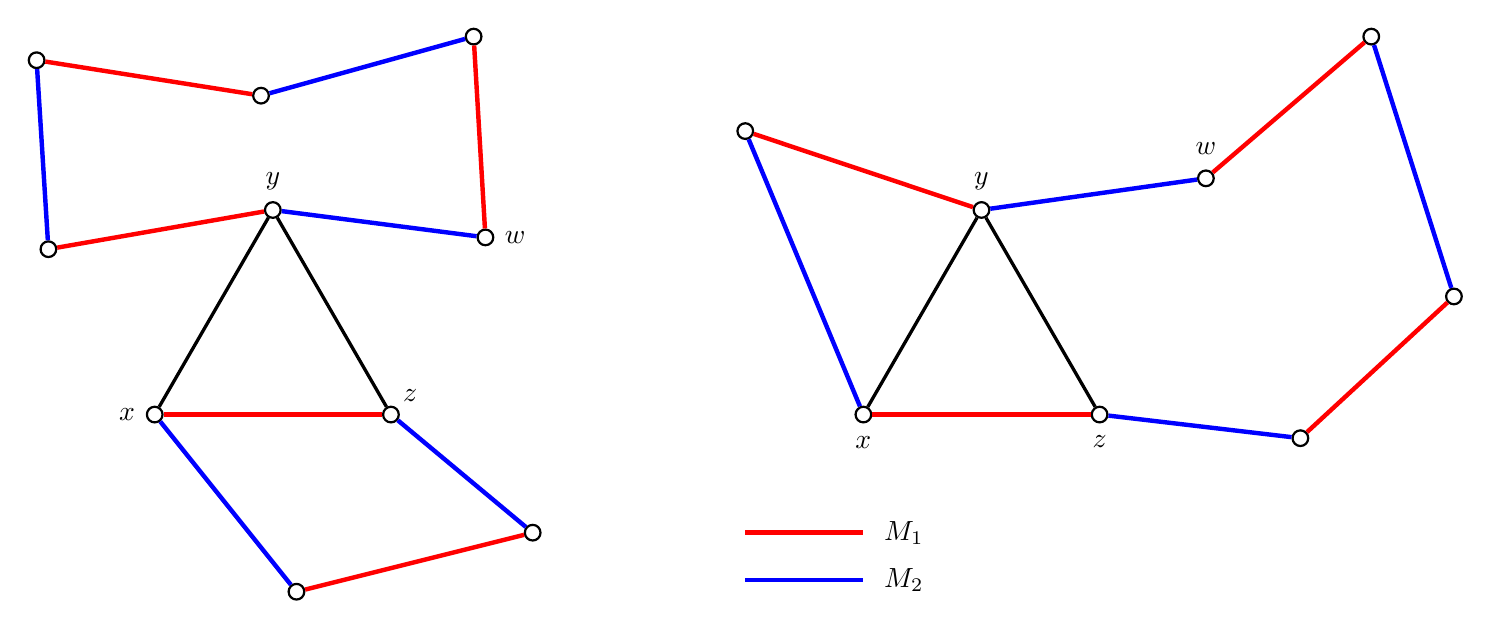
\begin{tikzpicture}[
    scale=1.5,
    every node/.style={draw,circle,thick,inner sep=2pt}
]

\begin{scope}
    % vertices.
    \node [label=above:$y$] (1) at (0, 1.732) {};
    \node [label=left:$x$] (2) at (-1, 0) {};
    \node [label=above right:$z$] (3) at (1, 0) {};
    \node (4) at (0.2, -1.5) {};
    \node (5) at (2.2, -1) {};
    \node [label=right:$w$] (6) at (1.8, 1.5) {};
    \node (7) at (1.7, 3.2) {};
    \node (8) at (-0.1, 2.7) {};
    \node (9) at (-2, 3) {};
    \node (0) at (-1.9, 1.4) {};
    % edges.
    \draw [very thick] (1) -- (2);
    \draw [very thick] (1) -- (3);
    \draw [ultra thick,red]  (2) -- (3);
    \draw [ultra thick,blue] (2) -- (4);
    \draw [ultra thick,red]  (4) -- (5);
    \draw [ultra thick,blue] (5) -- (3);
    \draw [ultra thick,blue] (1) -- (6);
    \draw [ultra thick,red]  (6) -- (7);
    \draw [ultra thick,blue] (7) -- (8);
    \draw [ultra thick,red]  (8) -- (9);
    \draw [ultra thick,blue] (9) -- (0);
    \draw [ultra thick,red]  (0) -- (1);
\end{scope}

\begin{scope}[xshift=6cm]
    % vertices.
    \node [label=above:$y$] (1) at (0, 1.732) {};
    \node [label=below:$x$] (2) at (-1, 0) {};
    \node [label=below:$z$] (3) at (1, 0) {};
    \node (4) at (2.7,-0.2) {};
    \node (5) at (4,1) {};
    \node (6) at (3.3,3.2) {};
    \node [label=above:$w$] (7) at (1.9,2) {};
    \node (8) at (-2,2.4) {};
    % edges.
    \draw [very thick] (1) -- (2);
    \draw [very thick] (1) -- (3);
    \draw [ultra thick,red]  (2) -- (3);
    \draw [ultra thick,blue] (3) -- (4);
    \draw [ultra thick,red]  (4) -- (5);
    \draw [ultra thick,blue] (5) -- (6);
    \draw [ultra thick,red]  (6) -- (7);
    \draw [ultra thick,blue] (7) -- (1);
    \draw [ultra thick,red]  (1) -- (8);
    \draw [ultra thick,blue] (8) -- (2);
\end{scope}

\begin{scope}[xshift=4cm,yshift=-1cm]
    \draw [ultra thick,red] (0,0) -- (1,0) node[draw=none,label=right:\color{black}$M_1$] {}; 
    \draw [ultra thick,blue] (0,-0.4) -- (1,-0.4) node[draw=none,label=right:\color{black}$M_2$] {};       
\end{scope}

\end{tikzpicture}

\end{document}
